\documentclass[11pt,a4paper,fontset=windows]{ctexart}
\usepackage[margin=2.5cm]{geometry}
\usepackage{amsmath,amssymb}
\usepackage{graphicx}
\usepackage{booktabs}
\usepackage{caption}
\usepackage{xcolor}
\usepackage{float}
\usepackage{newunicodechar}
\newunicodechar{μ}{\ensuremath{\mu}}
\usepackage[colorlinks=true,linkcolor=black,urlcolor=blue!60!black,citecolor=black]{hyperref}
\captionsetup{font=small,labelsep=quad}
\graphicspath{{figures/}}
\newcommand{\studentname}{[姓名]}
\newcommand{\pT}{p_{\mathrm{T}}}
\newcommand{\mll}{m_{\mu\mu}}
\newcommand{\GeV}{\,\mathrm{GeV}}
\ctexset{section={format=\Large\bfseries\raggedright},subsection={format=\large\bfseries\raggedright}}
\title{\bfseries 在 ATLAS 开放数据中重建 Z 玻色子\\[4pt]\large μ 子横动量阈值对不变质量分布的影响}
\author{\studentname\\[2pt]\small 暗物质课题学习组}
\date{2026 年 11 月}

\begin{document}
\maketitle

\begin{abstract}
本文用 ATLAS Open Data 2015 年 13~TeV 质子—质子对撞数据，从双 μ 子末态重建了 Z 玻色子。使用的是 \texttt{2muons} skim 的第一个文件，共 124935 个事件。无额外筛选时，核心区拟合给出峰位 $90.78\pm0.02\GeV$（仅统计误差）和分辨率 $\sigma=1.68\pm0.04\GeV$。提高 $\pT$ 阈值后，保留比例随质量明显上升：阈值接近 $m_Z/2\approx45.6\GeV$ 时事件数骤降，峰位也被推向高质量一侧。分析中还发现，教程 notebook 取前两个轻子的做法，在约 6.3\% 的事件中并不对应 μ 子对，本文对此作了修正。拟合峰位比已知 Z 质量低约 $0.41\GeV$；由于没有使用模拟样本，本文不能确定其来源。
\end{abstract}

\section{引言}

Z 玻色子是传递弱相互作用的中性规范玻色子，质量 $m_Z=91.1880\pm0.0020\GeV$，全宽 $\Gamma_Z=2.4955\pm0.0023\GeV$\cite{pdg}。由 $\tau=\hbar/\Gamma_Z$ 可知其寿命约 $2.6\times10^{-25}\,\mathrm{s}$，$c\tau$ 只有约 $0.08\,\mathrm{fm}$。所以探测器无法直接看到 Z，只能测量它的衰变产物。

本文研究 $Z\to\mu^+\mu^-$ 这一衰变道。μ 子能穿透量能器，在最外层的 μ 子谱仪中留下信号，本底相对较少。分析目标有三个：
\begin{enumerate}
  \item 跑通 ATLAS Open Data 教程 \emph{Find the Z boson}\cite{atlas}，由两个 μ 子重建 Z 的质量峰；
  \item 修改一个筛选条件（μ 子横动量阈值），比较修改前后的质量分布并解释变化；
  \item 明确只用数据、不用模拟时，哪些结论能下，哪些不能。
\end{enumerate}

\section{数据}

使用的数据版本是 \texttt{2025e-13tev-beta}，skim 为 \texttt{2muons}，质心能量 $\sqrt{s}=13\,\mathrm{TeV}$。该 skim 共 16 个文件，本文只用其中第一个：
\begin{center}
\texttt{ODEO\_FEB2025\_v0\_2muons\_data15\_periodD.2muons.root}
\end{center}
文件共 124935 个事件。教程的默认数据量是前一半（62467 个）。本文先用默认数据量复现教程结果，再扩大到整个文件。除非特别说明，下文数字都来自整个文件。全部 16 个文件尚未分析。

每个事件读取的变量是轻子的横动量 $\pT$、赝快度 $\eta$、方位角 $\phi$、能量 $E$、电荷和类型 \texttt{lep\_type}（13 表示 μ 子，11 表示电子），单位为 GeV。

\section{方法}

\subsection{不变质量}

探测器变量与直角坐标动量的关系是
\begin{equation}
p_x=\pT\cos\phi,\qquad p_y=\pT\sin\phi,\qquad p_z=\pT\sinh\eta .
\end{equation}
采用自然单位（$c=1$），两个 μ 子的不变质量定义为
\begin{equation}
\mll^2=(E_1+E_2)^2-\lvert\vec p_1+\vec p_2\rvert^2 .
\end{equation}
它是洛伦兹不变量，不依赖 Z 在实验室中的运动状态。如果两个 μ 子来自 Z 衰变，由四动量守恒可知 $\mll$ 就是该 Z 的质量。忽略 μ 子质量（$m_\mu\approx0.106\GeV\ll\pT$）时，
\begin{equation}
\mll^2\approx 2\,p_{\mathrm{T}1}\,p_{\mathrm{T}2}\left[\cosh(\eta_1-\eta_2)-\cos(\phi_1-\phi_2)\right],
\label{eq:massless}
\end{equation}
这个式子是后面解释阈值效应的关键。

\subsection{事件选择}

分析前先检查了数据结构，结果与教程注释不完全相符（表~\ref{tab:diagnostics}）：
\begin{itemize}
  \item skim 实际要求\textbf{至少}两个 μ 子，其中 99.0\% 的事件恰好有两个；
  \item 轻子数组里混有电子；
  \item 轻子不按 $\pT$ 排序（在前一半事件中，只有约 48\% 的事件按 $\pT$ 降序排列）。
\end{itemize}
教程直接取数组的前两个元素，因此在 7918 个事件（6.3\%）中，算出的并不是 μ 子对的质量。例如某事件的轻子依次为 $e$（$7.4\GeV$）、$\mu$（$40.4\GeV$）、$\mu$（$36.9\GeV$），教程算法得到 $14.9\GeV$，而两个 μ 子的不变质量是 $93.5\GeV$。

\begin{table}[H]
\centering
\caption{数据结构诊断（整个文件，共 124935 个事件）}
\label{tab:diagnostics}
\begin{tabular}{lr}
\toprule
检查项 & 事件数 \\
\midrule
恰有 2 个 μ 子 & 123670 \\
恰有 3 个 μ 子 & 1247 \\
恰有 4 个 μ 子 & 18 \\
\midrule
前两个轻子为 $\mu\mu$ & 117017 \\
前两个轻子为 $e\mu$ & 7066 \\
前两个轻子为 $ee$ & 852 \\
\bottomrule
\end{tabular}
\end{table}

因此本文改用如下选择：用 \texttt{lep\_type == 13} 选出 μ 子，每个事件取 $\pT$ 最高的两个。对有 3 个及以上 μ 子的事件（约 1\%），这一对不一定来自 Z。这样选出的 μ 子 $\pT$ 下限约为 $10\GeV$。

基准选择不加额外条件。对比研究中要求两个 μ 子都满足 $\pT>\pT^{\mathrm{cut}}$，$\pT^{\mathrm{cut}}$ 取 25、30、40、$45\GeV$。

\subsection{直方图与拟合}

直方图范围与教程相同，为 70--109~GeV（\texttt{np.arange(70,110,1)} 不含终点），每 bin 1~GeV，单 bin 误差取 $\sqrt{N}$。逐 bin 保留比例 $\varepsilon$ 的误差取二项误差 $\sqrt{\varepsilon(1-\varepsilon)/N_0}$，因为筛选后的事件是筛选前的子集，两者并不独立。

峰形用 Voigt 函数（Breit--Wigner 与高斯分辨率函数的卷积）加指数本底拟合：
\begin{equation}
f(m)=N\int \mathrm{BW}(m';\,m_{\mathrm{fit}},\Gamma_Z)\,G(m-m';\,\sigma)\,\mathrm{d}m'+B\,e^{-k(m-91)} .
\end{equation}
$\Gamma_Z$ 固定为 PDG 值，$N$、$m_{\mathrm{fit}}$、$\sigma$、$B$、$k$ 浮动，用最小二乘法分 bin 拟合。由于模型不含低质量一侧的拖尾，主拟合只取峰的核心区 85--97~GeV，再改变拟合范围检验其稳定性。

\subsection{交叉检查}

为确认本地计算与教程一致，我在本地按教程的 \texttt{calc\_mll}（\texttt{vector} 包）和相同的 \texttt{entry\_stop} 重算，得到 62467 个事件，窗口内 21475 个，峰值 bin 2657 个。按教程的画图代码重画后，与 notebook 中保存的图逐像素相同。本文的 numpy 公式与 \texttt{vector} 给出的总事件数相同，只有 2 个事件落入相邻 bin，这些事件紧贴 bin 边界，差别远小于统计误差。

人造数据测试复现了教程手算题的 $92.15\GeV$，并能从人造样本中还原设定的质量和分辨率。

\section{结果}

\subsection{质量谱与 Z 峰}

图~\ref{fig:spectrum} 是所选 μ 子对的完整质量谱。除 Z 峰外，还能看到与已知粒子质量相符的 $J/\psi$ 和 $\Upsilon$ 峰；图中标注是按已知质量给出的，本文没有单独验证这些低质量峰。

\begin{figure}[H]
\centering
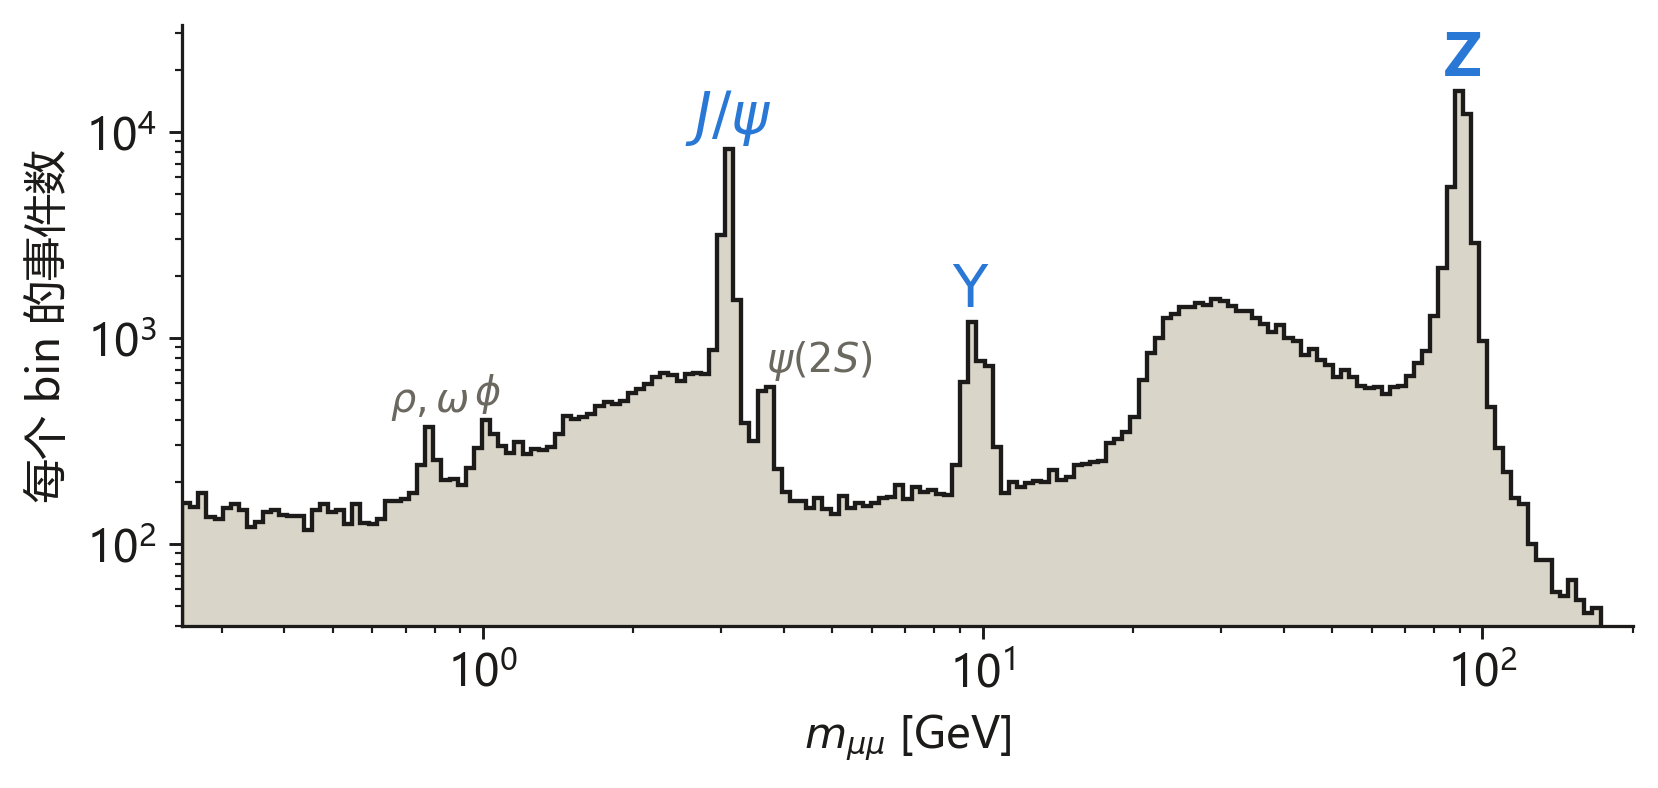
\includegraphics[width=0.92\linewidth]{spectrum.png}
\caption{整个文件的双 μ 子不变质量谱（双对数坐标）。}
\label{fig:spectrum}
\end{figure}

随着事件数增加，Z 峰从涨落中逐渐显现（图~\ref{fig:emergence}）。在无额外筛选时，70--109~GeV 窗口内共 43493 个事件，峰值位于 90.5~GeV 的 bin。

\begin{figure}[H]
\centering
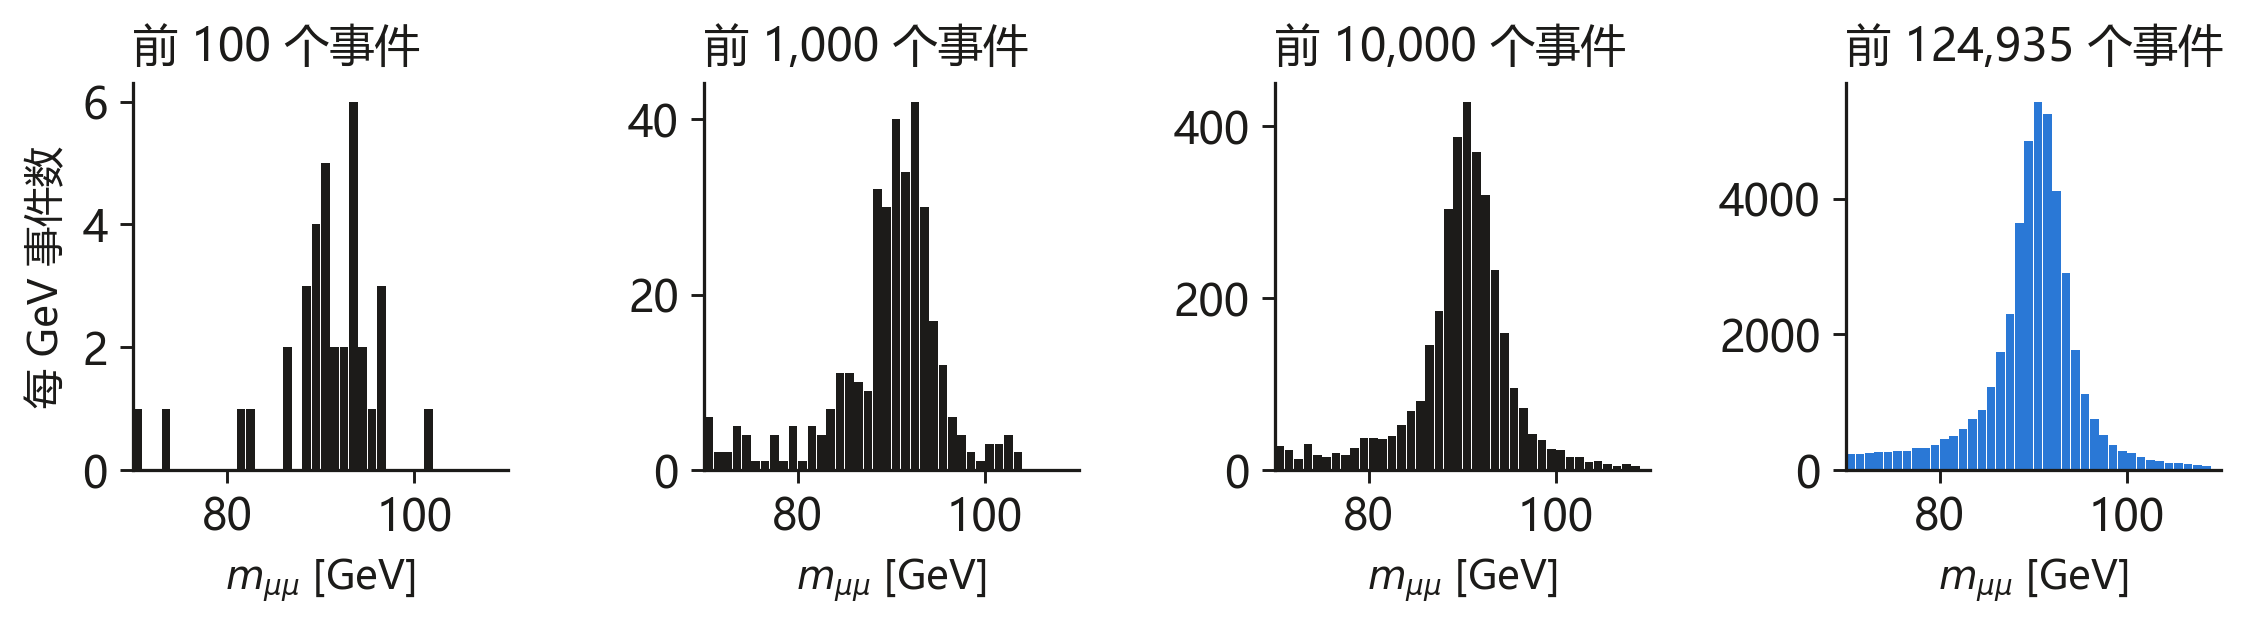
\includegraphics[width=\linewidth]{emergence.png}
\caption{按文件顺序累积事件时的质量分布。注意各图的纵轴范围不同。}
\label{fig:emergence}
\end{figure}

\subsection{修正事件选择的影响}

\begin{table}[H]
\centering
\caption{两种事件选择的比较（70--109~GeV 窗口）}
\label{tab:selection}
\begin{tabular}{lrr}
\toprule
选择方式 & 前一半事件 & 整个文件 \\
\midrule
教程：前两个轻子 & 21475 & 43084 \\
本文：两个 μ 子 & 21649 & 43493 \\
\bottomrule
\end{tabular}
\end{table}

修正后窗口内事件数只增加约 1\%（表~\ref{tab:selection}），所以教程的图依然能显示 Z 峰，这个问题单从峰形上很难察觉。

\subsection{改变 $\pT$ 阈值}

图~\ref{fig:comparison} 和表~\ref{tab:scan} 给出了阈值扫描的结果，表~\ref{tab:slices} 则按质量区间列出保留比例。

\begin{figure}[H]
\centering
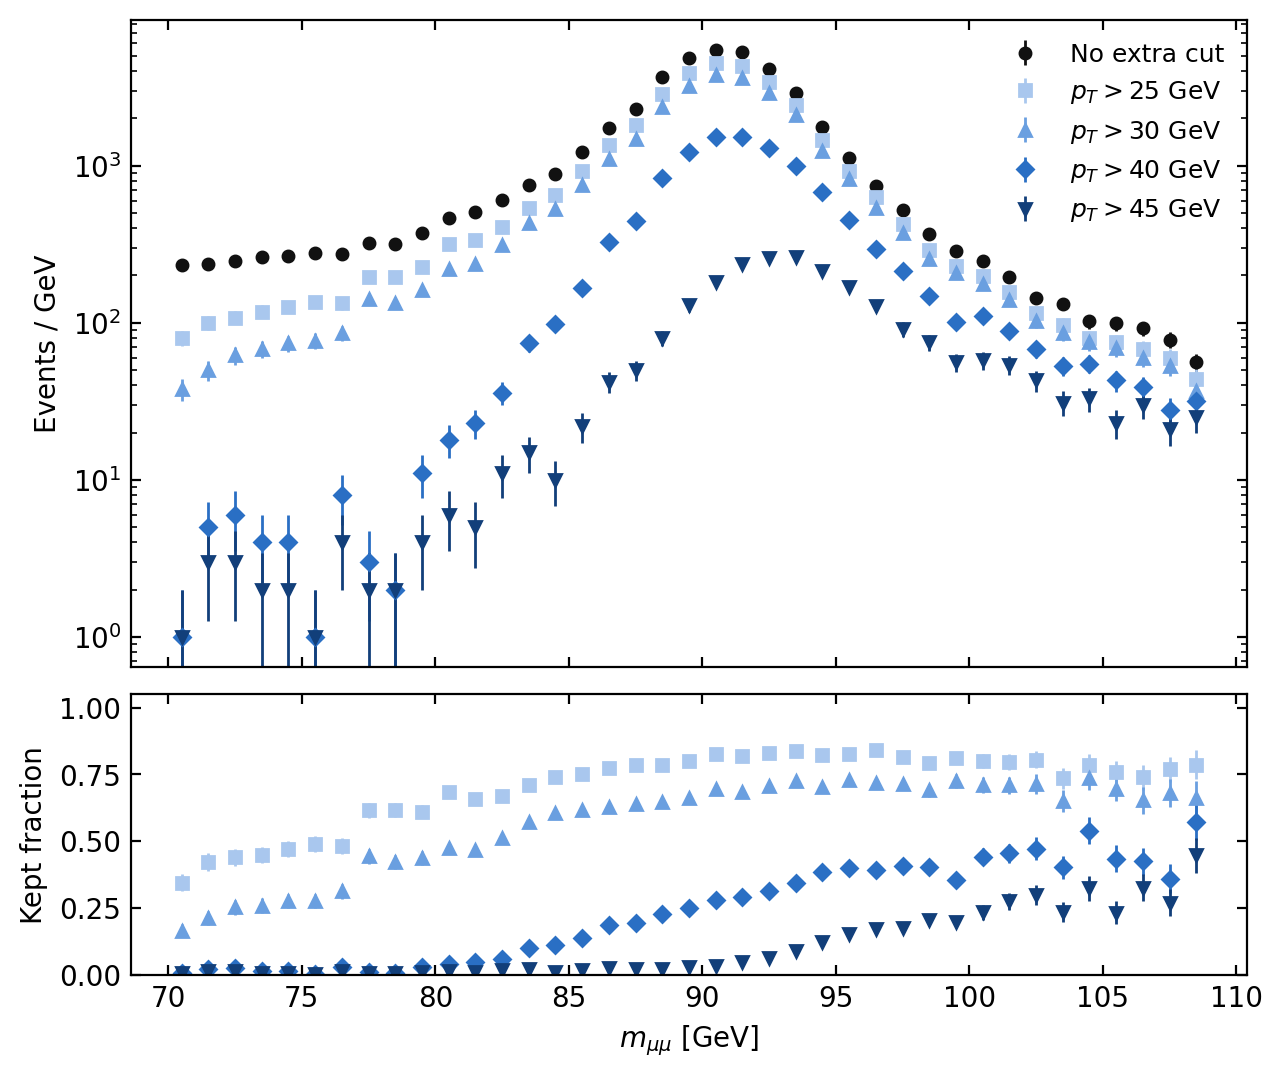
\includegraphics[width=0.78\linewidth]{../results/whole_first_file/cut_comparison.png}
\caption{不同 $\pT$ 阈值下的质量分布（上）和逐 bin 保留比例（下）。}
\label{fig:comparison}
\end{figure}

\begin{table}[H]
\centering
\caption{阈值扫描结果。拟合范围 85--97~GeV，误差仅含统计部分。}
\label{tab:scan}
\small
\begin{tabular}{rrrrccc}
\toprule
$\pT^{\mathrm{cut}}$ [GeV] & 事件数 & 保留比例 & 峰 bin [GeV] & $m_{\mathrm{fit}}$ [GeV] & $\sigma$ [GeV] & $\chi^2/\mathrm{ndf}$ \\
\midrule
\multicolumn{7}{l}{\emph{整个文件}} \\
无 & 43493 & 1 & 90.5 & $90.78\pm0.02$ & $1.68\pm0.04$ & 17.1/7 \\
25 & 34023 & 0.782 & 90.5 & $90.83\pm0.03$ & $1.66\pm0.04$ & 13.4/7 \\
30 & 28150 & 0.647 & 90.5 & $90.88\pm0.03$ & $1.66\pm0.04$ & 12.9/7 \\
40 & 11016 & 0.253 & 91.5 & $91.21\pm0.05$ & $1.74\pm0.10$ & 17.8/7 \\
45 & 2385 & 0.055 & 93.5 & $92.66\pm0.22$ & $1.95\pm0.26$ & 2.1/7 \\
\midrule
\multicolumn{7}{l}{\emph{前一半事件（教程默认数据量）}} \\
无 & 21649 & 1 & 90.5 & $90.77\pm0.04$ & $1.69\pm0.05$ & 10.3/7 \\
25 & 16909 & 0.781 & 90.5 & $90.83\pm0.04$ & $1.68\pm0.06$ & 4.3/7 \\
30 & 13997 & 0.647 & 90.5 & $90.89\pm0.04$ & $1.68\pm0.06$ & 5.8/7 \\
40 & 5555 & 0.257 & 90.5 & $91.25\pm0.08$ & $1.69\pm0.15$ & 11.6/7 \\
45 & 1227 & 0.057 & 92.5 & $93.1\pm2.2$ & $2.3\pm1.3$ & 1.7/7 \\
\bottomrule
\end{tabular}
\end{table}

\begin{table}[H]
\centering
\caption{不同质量区间的保留比例（整个文件）}
\label{tab:slices}
\begin{tabular}{lrrrrr}
\toprule
$\mll$ [GeV] & 70--80 & 80--88 & 88--94 & 94--100 & 100--109 \\
\midrule
基准事件数 & 2811 & 8484 & 26232 & 4818 & 1148 \\
$\pT>25\GeV$ & 0.51 & 0.75 & 0.82 & 0.82 & 0.78 \\
$\pT>30\GeV$ & 0.32 & 0.60 & 0.69 & 0.71 & 0.70 \\
$\pT>40\GeV$ & 0.016 & 0.14 & 0.28 & 0.39 & 0.45 \\
$\pT>45\GeV$ & 0.009 & 0.019 & 0.044 & 0.15 & 0.28 \\
\bottomrule
\end{tabular}
\end{table}

\subsection{峰位与分辨率}

无额外筛选时，拟合给出 $m_{\mathrm{fit}}=90.78\pm0.02\GeV$，$\sigma=1.68\pm0.04\GeV$，$\chi^2/\mathrm{ndf}=17.1/7$（图~\ref{fig:blur}）。对应的 Voigt 全宽约 $5.4\GeV$，明显大于 $\Gamma_Z$。

改变拟合范围后（表~\ref{tab:ranges}），峰位在 $90.63$--$90.78\GeV$ 之间变化，差异约 $0.15\GeV$，大于统计误差。范围越宽，$\chi^2/\mathrm{ndf}$ 越差。87--95~GeV 的拟合只有 3 个自由度，信号与本底难以分开，其结果不够稳定。

\begin{figure}[H]
\centering
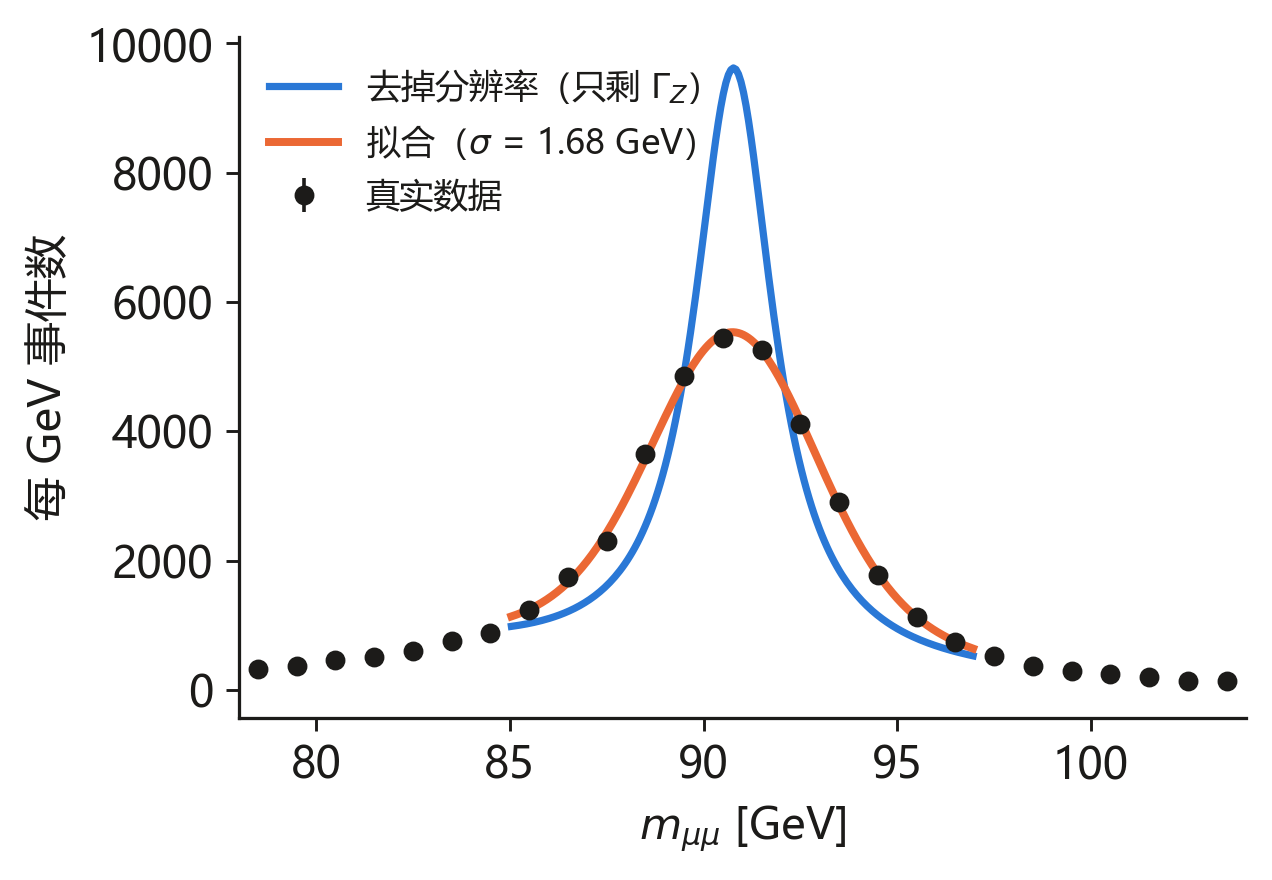
\includegraphics[width=0.68\linewidth]{blur.png}
\caption{无额外筛选时的 Z 峰。蓝线是把分辨率去掉、其余拟合参数不变时的形状，橙线是拟合结果。}
\label{fig:blur}
\end{figure}

\begin{table}[H]
\centering
\caption{拟合范围对结果的影响（整个文件，无额外筛选）}
\label{tab:ranges}
\begin{tabular}{lccc}
\toprule
拟合范围 [GeV] & $m_{\mathrm{fit}}$ [GeV] & $\sigma$ [GeV] & $\chi^2/\mathrm{ndf}$ \\
\midrule
87--95 & $90.72\pm0.17$ & $1.80\pm0.32$ & 4.2/3 \\
85--97（主拟合） & $90.78\pm0.02$ & $1.68\pm0.04$ & 17.1/7 \\
80--102 & $90.69\pm0.02$ & $1.84\pm0.02$ & 85.2/17 \\
75--105 & $90.63\pm0.02$ & $1.92\pm0.02$ & 272.4/25 \\
\bottomrule
\end{tabular}
\end{table}

\subsection{电荷检验}

Z 是电中性的，所以来自 Z 的两个 μ 子电荷必须相反。窗口内异号事件 42895 个，同号事件 598 个（1.4\%）。如图~\ref{fig:charge} 所示，同号分布在 Z 峰位置没有明显的峰，与预期相符。

\begin{figure}[H]
\centering
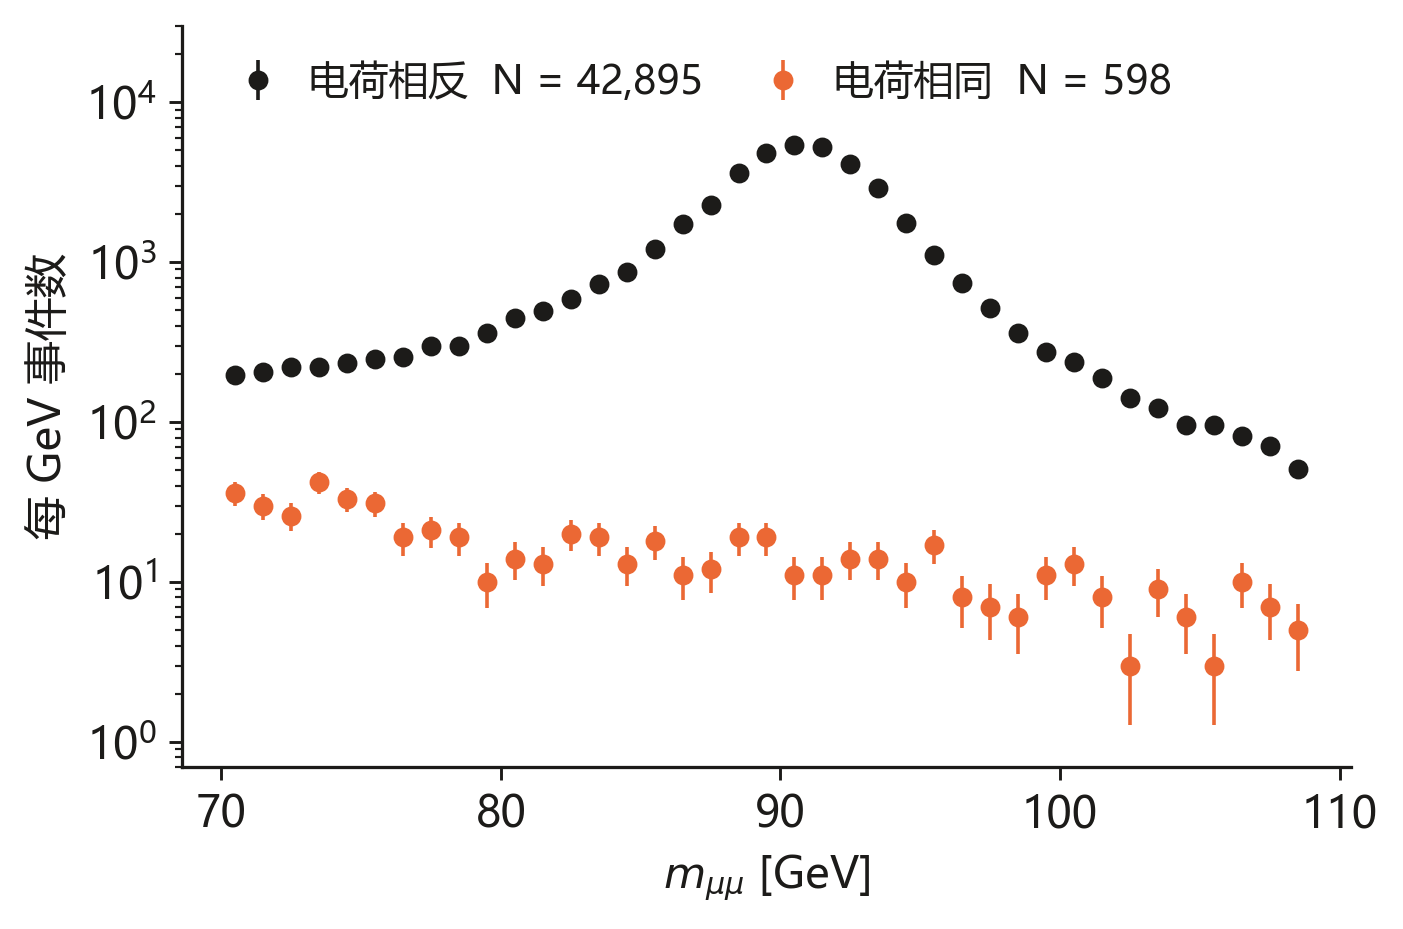
\includegraphics[width=0.62\linewidth]{charge.png}
\caption{异号与同号 μ 子对的质量分布。}
\label{fig:charge}
\end{figure}

\section{讨论}

\subsection{为什么低质量区保留得少}

由式~\eqref{eq:massless}，$\mll$ 小的事件，两个 μ 子的 $\pT$ 通常也小，因此更容易被阈值去掉。$\pT>30\GeV$ 时，70--80~GeV 只保留 32\%，而 88--94~GeV 保留 69\%。

\subsection{为什么 $45\GeV$ 附近事件骤减}

Z 静止时，两个 μ 子背对背，动量都等于 $m_Z/2\approx45.6\GeV$，所以 $\pT$ 不会超过这个值（$\pT=(m_Z/2)\sin\theta$）。把各向同性分布换算到 $\pT$，得到
\begin{equation}
\frac{\mathrm{d}N}{\mathrm{d}\pT}\propto\frac{\pT}{\sqrt{(m_Z/2)^2-\pT^2}},
\end{equation}
它在 $\pT\to m_Z/2$ 处发散，这就是 Jacobian 峰。实际分布被 Z 自身的横向运动和探测器分辨率抹平，并延伸到更高 $\pT$（图~\ref{fig:cliff} 左）；数据中的峰位略低于 $m_Z/2$，约在 42--$43\GeV$。保留比例在同一位置附近骤降（图~\ref{fig:cliff} 右）：85--97~GeV 内，阈值从 $40\GeV$ 升到 $46\GeV$，保留比例从 28\% 降到 3\%。

\begin{figure}[H]
\centering
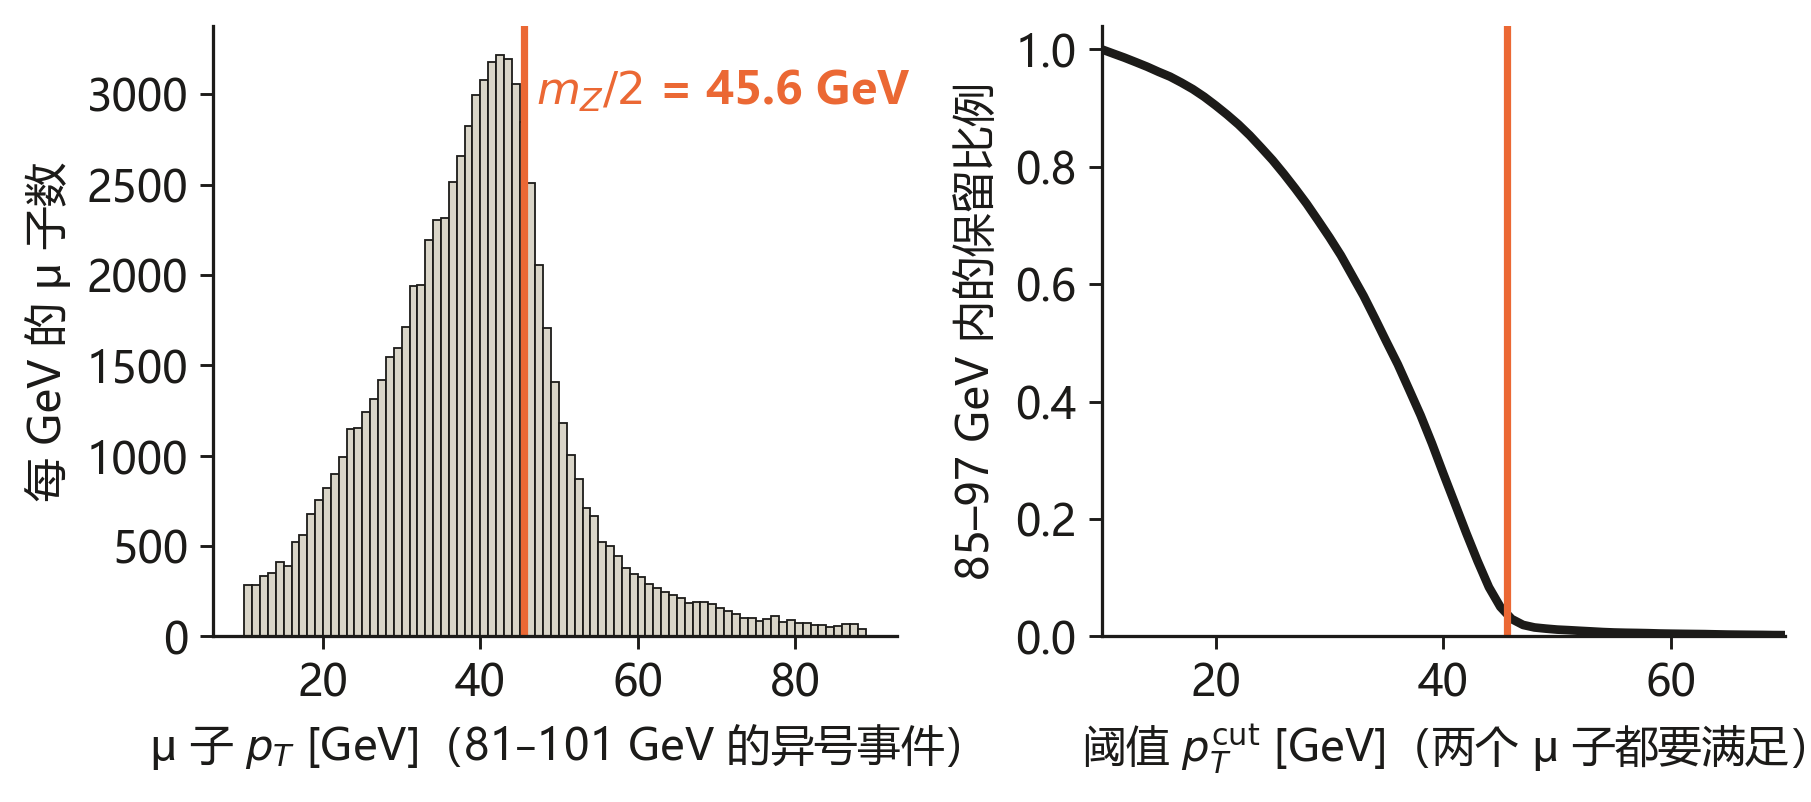
\includegraphics[width=\linewidth]{cliff.png}
\caption{左：Z 峰附近事件中 μ 子的 $\pT$ 分布。右：85--97~GeV 内的保留比例随阈值的变化。}
\label{fig:cliff}
\end{figure}

\subsection{峰位移动不代表 Z 的质量变了}

阈值升高时，低质量一侧先被切掉，峰位因此上移（图~\ref{fig:drift}）。这里有两个容易误读的地方：
\begin{itemize}
  \item $\pT>40\GeV$ 时拟合峰位为 $91.21\pm0.05\GeV$，几乎等于 PDG 值。但这只是峰位持续上移时恰好穿过了这个数，不能说明这个阈值测得更准。
  \item $\pT>45\GeV$ 时 $\chi^2/\mathrm{ndf}=2.1/7$，看起来很好，但这时事件少、误差大，分布已经被筛选扭曲，峰位 $92.66\GeV$ 不是 Z 质量的测量值。
\end{itemize}
所以 $\chi^2$ 好坏不足以判断结果是否有物理意义。此外，各阈值的事件是嵌套的子集，统计上并不独立，不能简单地把两行的误差合并来判断偏移的显著性。

\begin{figure}[H]
\centering
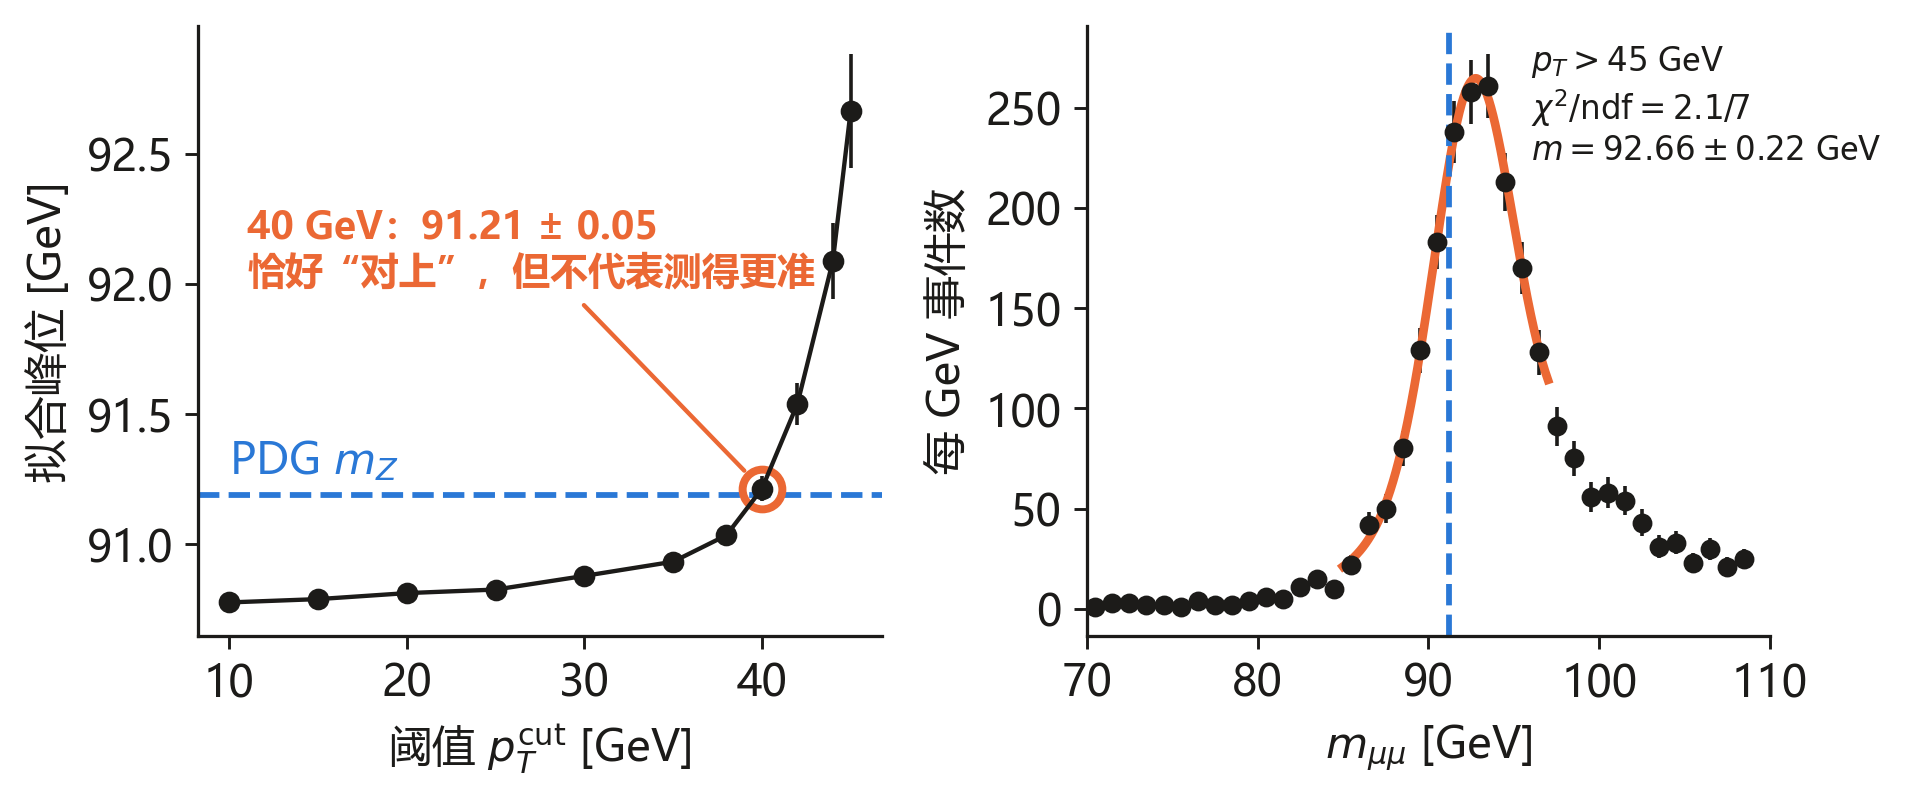
\includegraphics[width=\linewidth]{drift_trap.png}
\caption{左：拟合峰位随阈值的变化。右：$\pT>45\GeV$ 时的拟合。虚线为 PDG $m_Z$。}
\label{fig:drift}
\end{figure}

\subsection{观测宽度与峰位偏移}

观测到的全宽约 $5.4\GeV$，大于 $\Gamma_Z$，因为其中包含了探测器分辨率。拟合的 $\sigma\approx1.68\GeV$ 约为质量的 1.9\%。这个数字依赖拟合范围，在 $1.68$--$1.92\GeV$ 之间变化。

拟合峰位比 PDG 值低约 $0.41\GeV$（整个文件，主拟合），远大于统计误差，也大于拟合范围带来的差异。低质量一侧的拖尾（可能来自末态辐射）和 μ 子动量标度都可能造成这一偏移。\textbf{只靠这份数据无法区分这些原因}，本文也没有做系统误差分析，因此这一结果不应被视为 Z 质量的测量。

\subsection{阈值是否提高了信噪比}

$\pT$ 阈值从无到 $30\GeV$，88--94~GeV 与 70--80~GeV 的事件数之比从 9.3 升到 20.1，峰相对低质量区更突出了。但这个比值不等于信噪比 $S/B$：70--80~GeV 里也有 Z 的尾部，而 88--94~GeV 里也有非 Z 事件。没有本底模型时，只能定性地说峰更突出，不能给出 $S/B$。

\subsection{数据与模拟}

本文全程只用了数据。真实数据中，每个事件的来源是未知的，只能看统计分布。模拟（Monte Carlo）由事件产生器和探测器模拟生成，每个事件的来源是已知的。按截面和积分亮度归一化后，把各过程叠加与数据比较，才能把信号和本底分开、估计 $S/B$，并检验末态辐射等效应。本文无法回答的问题（如峰位为何偏低、窗口内本底占多少）都需要模拟或专门的校准研究。

\subsection{与暗物质课题的联系}

Z 还有约 20\% 的衰变是不可见的（$Z\to\nu\bar\nu$）\cite{pdg}，而本文只用了约 3.4\% 的 $Z\to\mu^+\mu^-$。对撞机上寻找暗物质的一类思路（mono-Z）也依赖重建 Z：寻找 $Z\to\ell\ell$ 伴随大丢失横能量 $E_{\mathrm{T}}^{\mathrm{miss}}$ 的事件。本文的方法正是这类分析的第一步。

作为示意，图~\ref{fig:met} 画出了 81--101~GeV 异号事件的 $E_{\mathrm{T}}^{\mathrm{miss}}$ 分布：共 39056 个事件，中位数 $25.1\GeV$，超过 $100\GeV$ 的有 114 个（0.29\%）。\textbf{这不是暗物质搜寻}：本文没有本底估计，也没有校验 $E_{\mathrm{T}}^{\mathrm{miss}}$ 的定义和校准，不能把尾部解读为信号。

\begin{figure}[H]
\centering
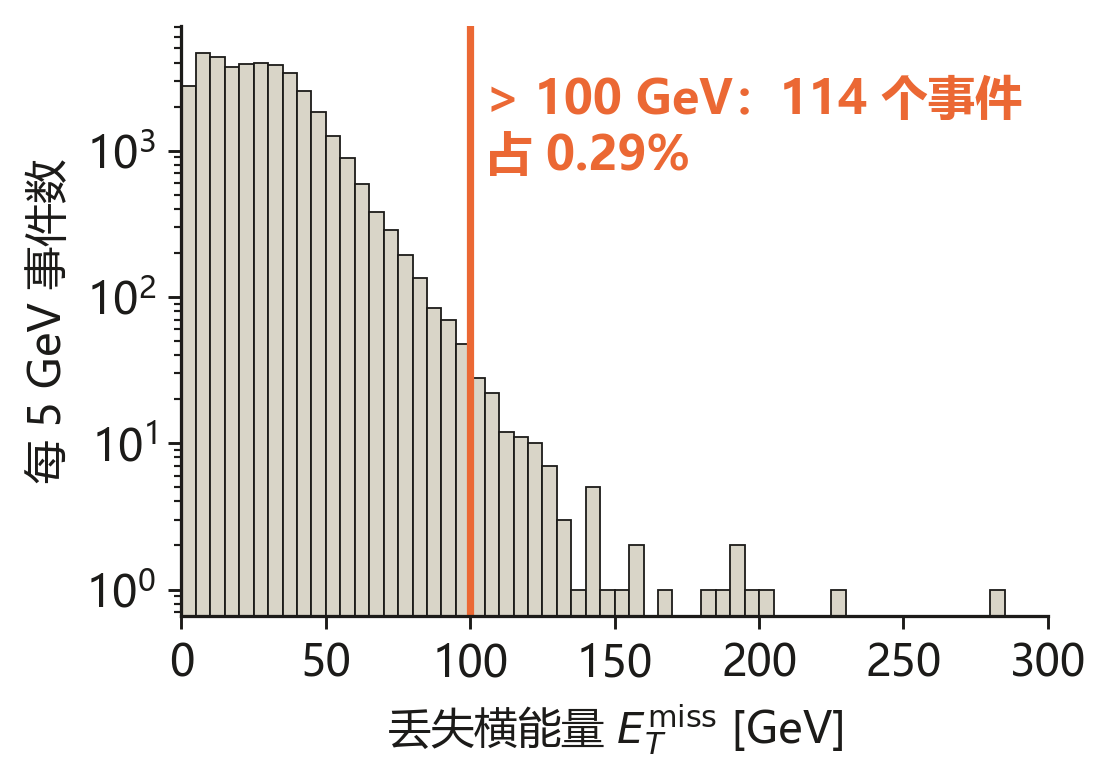
\includegraphics[width=0.62\linewidth]{met.png}
\caption{Z 峰附近异号事件的丢失横能量分布。}
\label{fig:met}
\end{figure}

\section{结论}

本文从 ATLAS 开放数据的双 μ 子事件中重建出了 Z 玻色子，峰位 $90.78\pm0.02\GeV$（仅统计误差），比已知值低约 $0.41\GeV$，来源尚不能确定。提高 $\pT$ 阈值时，低质量事件被优先去掉；阈值接近 $m_Z/2$ 时，事件数骤降，分布被明显扭曲，峰位随之上移。这一过程说明筛选条件不只是减少事件，也会改变分布的形状。此外，教程取前两个轻子的做法在约 6.3\% 的事件中并不对应 μ 子对，这提醒我们在使用数据前要先检查其结构。

下一步可以扩大到全部 16 个文件，并加入模拟样本，以分离信号与本底、检验峰位偏移的来源。

\appendix
\section{手算题}

\textbf{题 1：不变质量。} 由教程给出的四动量（单位 MeV），
\begin{gather*}
E=147913+21272=169185,\\
p_x=32387-18772=13615,\quad p_y=7047-9563=-2516,\quad p_z=144152-2942=141210,\\
M=\sqrt{E^2-p_x^2-p_y^2-p_z^2}\approx92150\,\mathrm{MeV}=92.15\GeV .
\end{gather*}

\textbf{题 2：洛伦兹因子。} 若 lep[0] 是电子，$\gamma=E/m=147913/0.5\approx3.0\times10^5$。

\textbf{题 3：总动量。} $\lvert\vec p_0\rvert=\sqrt{32387^2+7047^2+144152^2}\approx147913\,\mathrm{MeV}\approx147.9\GeV$，几乎等于 $E$。

\textbf{题 4：速度。} $\beta=p/E$，$\gamma\gg1$ 时 $1-\beta\approx1/(2\gamma^2)\approx6\times10^{-12}$。若用牛顿公式 $p=mv$，$v\le c$ 意味着 $p$ 最多约 $0.5\,\mathrm{MeV}$，比实际动量小约 30 万倍，所以必须使用相对论。

\section{概念题}

\textbf{Z 衰变为带电轻子的方式。} $Z\to e^+e^-$、$\mu^+\mu^-$、$\tau^+\tau^-$，分支比分别为 $(3.3632\pm0.0042)\%$、$(3.3662\pm0.0066)\%$、$(3.3696\pm0.0083)\%$\cite{pdg}。三者几乎相等，因为 Z 与三代轻子的耦合相同（轻子普适性）；轻子质量远小于 $m_Z$，相空间差异可以忽略。

\textbf{其他衰变方式。} 衰变为强子（$(69.911\pm0.056)\%$）和不可见末态（$(20.000\pm0.055)\%$，标准模型中对应中微子对）\cite{pdg}。

\section{复现方法}

分析在 Colab 跑通教程后，于本地环境完成：Python 3.9.6，uproot 5.6.9，awkward 2.8.12，vector 1.7.0，numpy 2.0.2，scipy 1.13.1，matplotlib 3.9.4。代码位于 \texttt{analysis/} 目录：\texttt{zll\_analysis.py} 负责筛选与拟合，\texttt{make\_figures.py} 负责作图，\texttt{crosscheck\_notebook.py} 负责与教程交叉检查，\texttt{test\_zll\_analysis.py} 用人造数据检查计算逻辑。

\begin{thebibliography}{9}
\bibitem{atlas} ATLAS Collaboration, ATLAS Open Data, \emph{Find the Z boson} 教程，\url{https://opendata.atlas.cern/docs/13TeV25Doc/StandardModel}。
\bibitem{pdg} S.~Navas \emph{et al.} (Particle Data Group), Phys.\ Rev.\ D \textbf{110}, 030001 (2024)，Z 玻色子条目。
\end{thebibliography}

\end{document}
